\section{Introduction}
\label{sec:introduction}

\begin{figure}[!htbp]
    \centering
    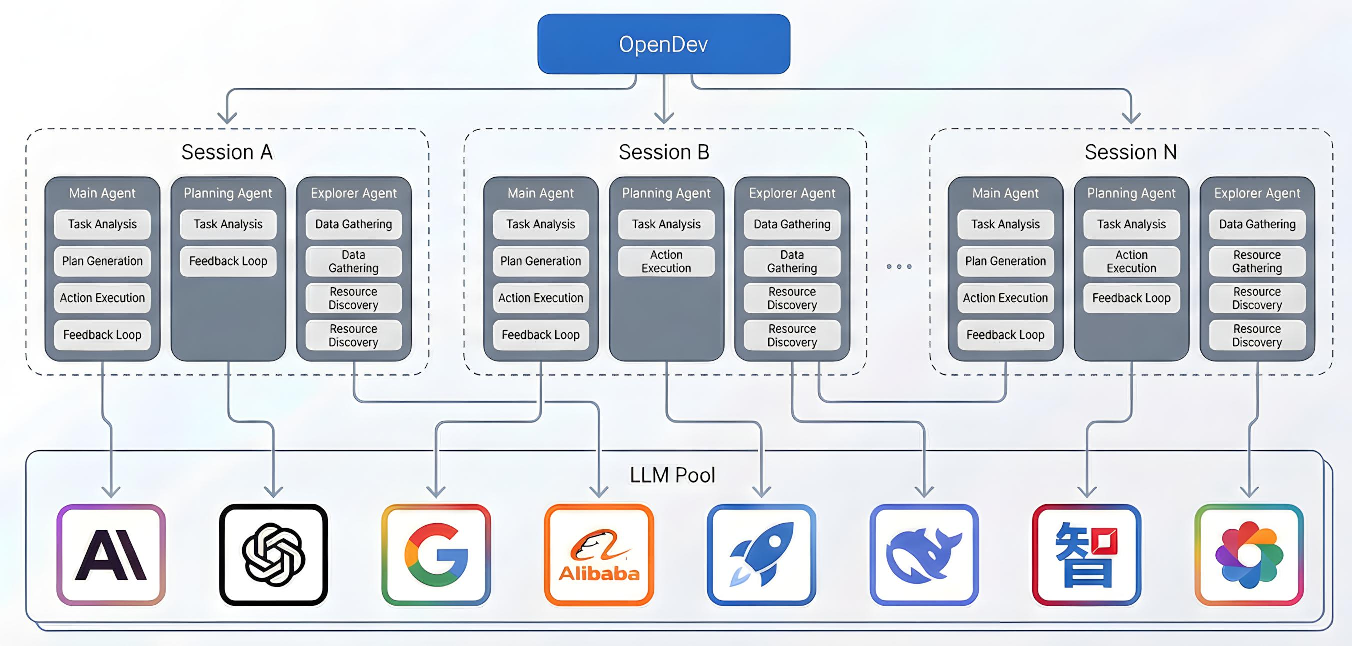
\includegraphics[width=\linewidth]{figures/top.pdf}
    \caption{Overview of \name. Work is organized into concurrent sessions, each composed of multiple specialized sub-agents; each agent executes typed workflows (Execution, Thinking, Compaction) that independently bind to a user-configured LLM. This four-level hierarchy (session $\to$ agent $\to$ workflow $\to$ LLM) enables fine-grained model selection, allowing cost, latency, and capability trade-offs to be optimized per workflow.}
    \label{fig:top}
\end{figure}

The rapid advancement of large language models (LLMs) has catalyzed a new paradigm in software development: AI-powered coding assistants that operate as autonomous agents~\cite{yang2024swe, zhang2025adaptive, yao2023react}. Unlike traditional code completion tools that suggest inline snippets, agentic coding assistants can reason about complex tasks, execute multi-step plans, and interact with the development environment through tool use. Comprehensive surveys have documented the explosive growth of code intelligence research~\cite{code_survey, issue_resolution_survey}, and roadmaps for Agentic Software Engineering~\cite{sase_survey} have formalized the methodological principles governing human--AI collaboration. Systems such as SWE-Agent~\cite{yang2024swe}, OpenHands~\cite{openhands}, and HyperAgent~\cite{phan2024hyperagent} have demonstrated the potential of autonomous agents on standardized benchmarks. The commercial impact has been equally dramatic, with GitHub Copilot surpassing 15 million developers~\cite{github2025copilot_agent}, rapid revenue growth for AI-native editors~\cite{cursor2025}, and major labs launching autonomous coding agents~\cite{cognition2024devin, openai2025codex}, signaling that agentic coding has moved from research prototype to industrial deployment.

\paragraph{The rise of terminal-native agents.} For the past few years, AI coding assistants have been tightly integrated into IDEs, acting as reactive copilots requiring constant human oversight. Recently, a major shift has begun, moving away from complex IDE plugins toward simpler command-line interfaces. Claude Code~\cite{anthropic2025claudecode} led this shift, demonstrating that a terminal-native agent could match or exceed IDE-integrated tools in real-world software engineering tasks. The terminal is the operational heart of software development, natively supporting source control, build systems, remote SSH sessions, and headless server environments. Early systems such as Aider~\cite{aider2024}, CodeAct~\cite{wang2024codeact}, and Open Interpreter~\cite{openInterpreter} demonstrated the viability of terminal-based AI pair programming and executable code actions. Today, every major AI lab offers a CLI agent~\cite{anthropic2025claudecode, google2025geminicli, openai2025codex}, alongside open-source alternatives such as Goose~\cite{block2025goose}, OpenCode~\cite{opencode2025}, and Crush~\cite{charmbracelet2025crush}. However, realizing this potential is non-trivial. Benchmarks such as Terminal-Bench~\cite{terminal_bench} and LongCLI-Bench~\cite{longcli_bench} demonstrate that even frontier models struggle with continuous terminal operation, underscoring the need for purpose-built engineering solutions.

These benchmark results point to three fundamental engineering challenges that any long-running terminal agent must solve: managing finite context windows over sessions that routinely exceed the model's token budget, preventing destructive operations when the agent can execute arbitrary shell commands, and extending capabilities without overwhelming the agent's prompt budget. We organize the architectural response around two phases: \emph{scaffolding}, which assembles the agent (system prompt, tool schemas, subagent registry) before the first prompt, and the \emph{harness}, which orchestrates tool dispatch, context management, and safety enforcement at runtime~\cite{anthropic2025harness} (\Cref{sec:agent_core}). Yet the design space for terminal-native agentic tools remains largely underexplored: most production systems are closed-source with undocumented architectural decisions, and existing open-source frameworks either target benchmarks rather than interactive use or lack published technical reports~\cite{mei2025survey, hua2025context}. Three critical open questions motivate this work: How should multi-model architectures balance cost, latency, and capability across different cognitive tasks? What safety mechanisms prevent destructive operations without hampering developer productivity? And how can systems sustain long-running conversations within finite context limits?

In this paper, we present \name, an open AI-powered command-line agent for software engineering. To the best of our knowledge, this is the first comprehensive technical report for an open-source, terminal-native, interactive coding agent. Existing systems occupy one of two categories: benchmark-oriented frameworks such as SWE-Agent~\cite{yang2024swe} have published research papers but are primarily designed for automated evaluation rather than interactive daily use; OpenHands~\cite{openhands} is both production-grade and well-documented but operates through a browser-based UI rather than a terminal interface; CLI-native agents such as Aider~\cite{aider2024}, Goose~\cite{block2025goose}, OpenCode~\cite{opencode2025}, Crush~\cite{charmbracelet2025crush}, and Gemini CLI~\cite{google2025geminicli} lack published technical reports documenting their design decisions; and Claude Code~\cite{anthropic2025claudecode} is CLI-native but neither open-source nor accompanied by a published technical report. \textbf{The purpose of this paper is not to present a novel algorithmic breakthrough, but rather to share the design decisions, trade-offs, and lessons learned from engineering a production-ready, agentic coding system that bridges the gap between closed-source industrial practice and open academic discourse.}

A central design principle of \name is that it is a \textbf{compound AI system}~\cite{zaharia2024compound}: not a single monolithic LLM, but a structured ensemble of agents and workflows, each independently bound to a user-configured LLM (\Cref{sec:multi_model}). This framing, articulated by Zaharia et al., argues that state-of-the-art AI results are increasingly achieved by systems that compose multiple models, retrievers, and tools rather than relying on a single model call. \name operationalizes this principle: its decoupled architecture makes the system model-agnostic by construction, and techniques like learned model routing~\cite{ong2024routellm} can be applied at the workflow level. Switching providers or optimizing cost requires only a configuration change, not a code change. The system's capabilities are therefore not fixed at deployment but continuously upgradeable as better models emerge.

\paragraph{Design principles and contributions.} The design of \name is guided by three overarching principles. First, \emph{separation of concerns}: each architectural decision (model selection, context management, safety enforcement, tool dispatch) should be independently configurable and replaceable without affecting the others. Second, \emph{progressive degradation}: the system should function gracefully as resources are exhausted, whether that means token budget, iteration count, or network connectivity. Third, \emph{transparency over magic}: every system action (tool calls, safety vetoes, context compaction, memory updates) should be observable and overridable by the developer. These principles manifest in five concrete contributions:

\begin{packedenumerate}
\item \textbf{Per-workflow LLM configurability via a compound architecture.} Different execution phases impose different demands on model capability, latency, and cost. We present a per-workflow LLM binding architecture where each cognitive workflow independently selects a model via user configuration (\Cref{sec:multi_model}), informed by the compound AI systems perspective~\cite{zaharia2024compound} and model routing research~\cite{ong2024routellm}.

\item \textbf{Extended ReAct execution pipeline.} We extend the standard ReAct cycle~\cite{yao2023react} with explicit thinking and optional self-critique phases that separate deliberation from action (hereafter, the \emph{ReAct loop}; \Cref{sec:react_executor}), and integrate staged context compaction directly into the reasoning loop, drawing on insights from context engineering research~\cite{mei2025survey, hua2025context}.

\item \textbf{Behavioral steering over long horizons.} We present event-driven system reminders that counteract instruction fade-out in long-running sessions by injecting targeted guidance at the point of decision rather than relying solely on the initial system prompt (\Cref{sec:system_reminders}). A conditional prompt composition pipeline assembles agent instructions from independent, priority-ordered sections that load only when contextually relevant, reducing prompt overhead while preserving comprehensive guidance (\Cref{sec:prompt_composition}).

\item \textbf{Token-efficient extensibility and defense-in-depth safety.} We present a registry-based tool architecture with lazy-discovered external tools via MCP~\cite{anthropic2024mcp} (\Cref{sec:mcp}) and a five-layer safety architecture that enforces constraints at progressively lower levels of abstraction: prompt-level guardrails, schema-level tool gating through dual-agent separation (\Cref{sec:agent_core}), a runtime approval system with persistent permissions, tool-level validation, and user-defined lifecycle hooks (\Cref{sec:safety_architecture}).

\item \textbf{Context engineering as a first-class concern.} We treat context management as a first-class engineering concern~\cite{anthropic2025context_engineering, mei2025survey}, presenting Adaptive Context Compaction (\Cref{sec:adaptive_compaction}), event-driven system reminders to counteract attention decay (\Cref{sec:system_reminders}), and an experience-driven memory pipeline~\cite{packer2023memgpt, experepair} that accumulates project-specific knowledge. Our compaction and memory strategies align with the entropy-reduction and minimal-sufficiency principles identified in recent theoretical work on context engineering~\cite{hua2025context, ye2026meta}.
\end{packedenumerate}

\paragraph{Paper organization.} The remainder of this paper follows the path from construction to reflection to context. \Cref{sec:architecture} details what was built: the four-layer system architecture spanning agent reasoning, context engineering, tooling, and persistence. \Cref{sec:discussion} examines what was learned: five cross-cutting design tensions that emerged during iterative development and the transferable lessons they yield. \Cref{sec:related_work} positions these decisions within the broader research landscape, and \Cref{sec:conclusion} identifies future directions. The appendix provides reference-level catalogs of tools, prompts, configuration schemas, and implementation constants.
